\documentclass[tikz]{standalone}
\usepackage{pgfplots}
\pgfplotsset{compat=1.15}
\usepackage{mathrsfs}
\usetikzlibrary{arrows,calc}
\usepackage{tkz-euclide}

\pagestyle{empty}

\definecolor{AngleClr}{rgb}{0,0.39215686274509803,0}
\definecolor{ShapeClr}{rgb}{0.6,0.2,0}

\begin{document}

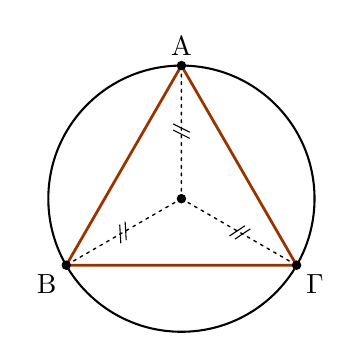
\begin{tikzpicture}[scale=.75]
\tkzSetUpLine[line width=1pt,color=black]
\tkzSetUpPoint[fill=black]

\tkzDefPoints{0/0/B,1.95/3.38/A,3.9/0/C}

\tkzDefCircle[in](A,B,C)\tkzGetPoint{I}
\tkzDefPointBy[projection=onto A--B](I) \tkzGetPoint{Ic}
\tkzDefPointBy[projection=onto B--C](I) \tkzGetPoint{Ia}
\tkzDefPointBy[projection=onto C--A](I) \tkzGetPoint{Ib}

\tkzFillPolygon[fill=white](A,B,C)


\tkzDrawSegments[line width=0.5pt,color=black,dashed,dash pattern=on 1pt off 1.75pt](I,A I,B I,C)

\tkzDrawCircle[color=black,line width=0.75pt](I,A)

\tkzDrawPolygon[color=ShapeClr](A,B,C)
\tkzDrawPoints[size=3](A,B,C,I)
\tkzLabelPoint[above](A){$\rm A$}
\tkzLabelPoint[below left](B){$\rm B$}
\tkzLabelPoint[below right](C){$\rm \Gamma$}

\tkzMarkSegments[mark=s||,size=3](I,A I,B I,C)

\end{tikzpicture}

\end{document}
